\documentclass[12pt, letterpaper]{article}

\usepackage[margin=1in]{geometry}
\usepackage{amsmath}
\usepackage{graphicx}
\usepackage{hyperref}
\hypersetup{
    colorlinks=true,
    linkcolor=blue,
    filecolor=magenta,      
    urlcolor=cyan,
}

\begin{document}

\section*{1D Kinematics}
\begin{align}
  v_f = v_0 + at \\
  \Delta x = \frac{\Delta v}{2}t \\
  \Delta x = v_0t + \frac{a}{2}t^2 \\
  v_f^2 = v_0^2 + 2a\Delta x
\end{align}

\section*{2D Projectile}
\begin{align}
  t_f = \frac{2v_0\sin{(\theta)}}{g} \\
  t_f = \frac{v_0\sin{(\theta)} + \sqrt{v_0^2\sin^2{(\theta)} + 2gy_0}}{g} \\
  R = \frac{v_0^2 \sin{(2\theta)}}{g} \\
  R = \frac{v_0\cos{(\theta)}}{g}\biggl(v_0\sin{(\theta)} + \sqrt{v_0^2\sin^2{(\theta)} + 2gy_0}\biggr) \\
  R = \sin{(2\theta)}\frac{v_0^2}{2g}\biggl(1 + \sqrt{1 + \frac{2gy_0}{v_0^2\sin^2{(\theta)}}}\biggr) \\
  H_{max} = y_0 + \frac{v_0^2\sin^2{(\theta)}}{2g} \\
  \theta = \frac{1}{2}\arcsin{\biggl(\frac{g\Delta x}{v_0^2}\biggr)} \\
  \theta = 90 - \frac{1}{2}\arcsin{\biggl(\frac{g\Delta x}{v_0^2}\biggr)} \\
  \theta = \arctan{\biggl(\frac{y_f}{x_f} + \sqrt{\frac{y_f^2}{x_f^2}+1}\biggr)} \\
  v_0 = \sqrt{\frac{x^2g}{x\sin{(2\theta)} - 2y\cos^2{(\theta)}}}
\end{align}

\section*{Circular Motion}
\begin{align}
  a_{tot} = \sqrt{a_r^2 + a_t^2} \\
  \omega = \frac{2\pi}{T} \\
  v = \omega r \\
  a_r = \omega^2r \\
  a_r = \frac{v^2}{r} \\
  F_c = a_rm \\
  \alpha = \frac{a_t}{r}
\end{align}

One can use all of the 1D Kinematics equations with:
\begin{align*}
  x = \theta \\
  v_i = \omega_i \\
  a = \alpha
\end{align*}

\section*{Forces}
\begin{align}
  \Sigma \vec{F} = m \vec{a}
\end{align}

\section*{Energy}
\begin{align}
  K = \frac{1}{2}mv^2 \\
  K = \frac{1}{2}I\omega^2 \\
  U = mgh \\
  U = \frac{1}{2}kx^2 \\
  U = mgy_{cm} \\
  E_{th} = fs \\
  W = F \cdot D = \lvert F \rvert \lvert D \rvert \cos{(\theta)} \\
  F \cdot D = F_xD_x + F_yD_y ...
\end{align}

\section*{Momentum}
\begin{align}
  \Delta\rho = J \\
  J = \int F(t)dt \\
  \text{Elastic} \\
  v_1 = \frac{m_1-m_2}{m_1+m_2}u_1 + \frac{2m_2}{m_1+m_2}u_2 \\
  v_2 = \frac{m_1-m_2}{m_1+m_2}u_2 + \frac{2m_1}{m_1+m_2}u_1 \\
  \text{Inelastic Stick} \\
  v = \frac{m_1}{m_1+m_2}u_1
\end{align}

\section*{Moment of Inertia}
\begin{align}
  x_{cm} = \frac{\sum mx}{\sum m} \\
  I = I_{cm} + Md^2 \\
  I_{disk} = \frac{1}{2}mr^2 \\
  I_{hoop} = mr^2 \\
  I_{sphere} = \frac{2}{5}mr^2 \\
  I_{sphere\_hollow} = \frac{2}{3}mr^2 \\
  I_{rod\_center} = \frac{1}{12}ml^2 \\
  I_{rod\_end} = \frac{1}{3}ml^2
\end{align}

\section*{Torque}
\begin{align}
  \tau = rF\sin{(\theta)} \\
  \tau = r \times F = rF\sin{(\theta)} \\
  \tau = r_{moment}F \\
  \tau = I\alpha \\
  P = \tau\omega
\end{align}

\section*{Angular Momentum}
\begin{align}
  L = \rho \times r \\
  L = I\omega
\end{align}

\section*{Gravity}
\begin{align}
  G = 6.67 \cdot 10^{-11} \\
  F_g = \frac{GMm}{r^2} \\
  U = -\frac{GMm}{r} \\
  K = \frac{GMm}{2r} \\
  E = -\frac{GMm}{2r} \\
  v_{esc} \geq \sqrt{\frac{2GM}{r}} \\
  v = \sqrt{\frac{GM}{r}} \\
  T = 2\pi\sqrt{\frac{a^3}{GM}}
\end{align}

\section*{Simple Harmonic Motion}
\begin{align}
  F = -kx \\
  \omega = \sqrt{\frac{k}{m}} \\
  x(t) = x_0\cos{\left (\sqrt{\frac{k}{m}}t \right)} + \frac{v_0}{\sqrt{\frac{k}{m}}}\sin{\left( \sqrt{\frac{k}{m}}t  \right)} \\
  x(t) = A\cos{(\omega t - \phi)} \\
  c_1 = x_0 \\
  c_2 = \frac{v_0}{\omega} \\
  \tan{(\phi)} = \frac{c_1}{c_2} \\
  v = \omega \sqrt{A^2 - x^2} \\
  a = \omega^2 A
  K(t) = \frac{1}{2}kA^2\sin^2(\omega t - \phi) \\
  U(t) = \frac{1}{2}kA^2\cos^2(\omega t - \phi) \\
  E = \frac{1}{2}kA^2 \\
  T = 2\pi \sqrt{\frac{l}{g}} \\
  \omega = \sqrt{\frac{mgl}{I}}
\end{align}

\section*{Fluids}
\begin{align}
  \rho = \frac{m}{V} \\
  p = \frac{F}{A} \\
  F_b = \rho g V \\
  v_1A_1 = v_2A_2 \\
  p = \rho gd + P_0 \\
  P_1 + \frac{1}{2}\rho v_1^2 + \rho g y_1 = P_2 + \frac{1}{2}\rho v_2^2 + \rho g y_2
\end{align}

\section*{Thermodynamics}
\begin{align}
  R = 8.314 \\
  N_{av} = 6.022 \cdot 10^{23} \\
  k_B = 1.38 \cdot 10^{-23} \\
  pV = nRT \\
  pV = Nk_BT \\
  pV^\gamma = constant \\
  TV^{\gamma - 1} = constant \\
  \gamma = \frac{C_p}{C_v} \\
  C_p = C_v + R \\
  \Delta E = W + Q \\
  \Delta E = nC_v\Delta T \\
  Q = nC_x\Delta T \\
  \eta = \frac{W_{out}}{Q_H} \\
  W_{out} = Q_H - Q_C \\
  \eta_{carnot} = 1 - \frac{T_C}{T_H} \\
  K = \frac{Q_C}{W_{in}} \\
  Q_H = Q_C + W_{in} \\
  K_{carnot} = \frac{T_C}{T_H - T_C}
\end{align}

\section*{Special Relativity}
\begin{align}
  \gamma = \frac{1}{\sqrt{1-\frac{v^2}{c^2}}} \\
  \frac{v}{c} = \frac{1}{\sqrt{1-\frac{1}{\gamma^2}}} \\
  \Delta t = \gamma\Delta\tau \\
  L = \frac{L_0}{\gamma} \\
  s^2 = c^2(\Delta t)^2 - (\Delta x)^2 \\
  s^2 = s\prime^2 \\
  x\prime = \gamma(x - vt) \\
  t\prime = \gamma(t - \frac{vx}{c^2}) \\
  x = \gamma(x\prime + vt\prime) \\
  t = \gamma(t\prime + \frac{vx\prime}{c^2}) \\
  u\prime = \frac{u - v}{1-\frac{uv}{c^2}} \\
  u = \frac{u\prime + v}{1+\frac{u\prime v}{c^2}} \\
  \rho = \gamma_\rho mu \\
  E = E_0 + K = \gamma_\rho mc^2 \\
  E_0 = mc^2 \\
  K = (\gamma_\rho - 1)mc^2 \\
  E^2 = E_0^2 + (pc)^2
\end{align}

\section*{Periodic Table}
\url{https://www.thoughtco.com/thmb/67-ZE4diyATe7qUfN0zBNfZ-gH0=/1920x0/filters:no_upscale():max_bytes(150000):strip_icc():format(webp)/PeriodicTableoftheElements-5c3648e546e0fb0001ba3a0a.jpg}

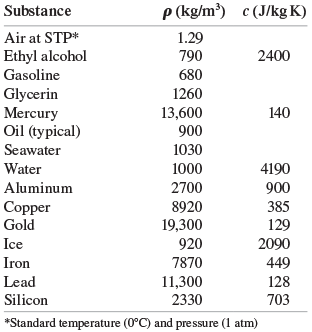
\includegraphics{densities}

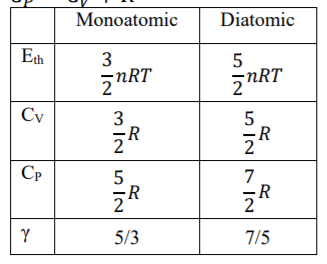
\includegraphics[width=15cm]{thermo_constants}

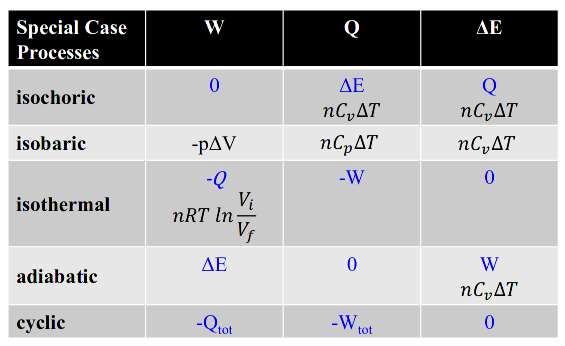
\includegraphics{thermo_procedures}

\end{document}
